\documentclass[twoside]{book}

% Packages required by doxygen
\usepackage{fixltx2e}
\usepackage{calc}
\usepackage{doxygen}
\usepackage[export]{adjustbox} % also loads graphicx
\usepackage{graphicx}
\usepackage[utf8]{inputenc}
\usepackage{makeidx}
\usepackage{multicol}
\usepackage{multirow}
\PassOptionsToPackage{warn}{textcomp}
\usepackage{textcomp}
\usepackage[nointegrals]{wasysym}
\usepackage[table]{xcolor}

% Font selection
\usepackage[T1]{fontenc}
\usepackage[scaled=.90]{helvet}
\usepackage{courier}
\usepackage{amssymb}
\usepackage{sectsty}
\renewcommand{\familydefault}{\sfdefault}
\allsectionsfont{%
  \fontseries{bc}\selectfont%
  \color{darkgray}%
}
\renewcommand{\DoxyLabelFont}{%
  \fontseries{bc}\selectfont%
  \color{darkgray}%
}
\newcommand{\+}{\discretionary{\mbox{\scriptsize$\hookleftarrow$}}{}{}}

% Page & text layout
\usepackage{geometry}
\geometry{%
  a4paper,%
  top=2.5cm,%
  bottom=2.5cm,%
  left=2.5cm,%
  right=2.5cm%
}
\tolerance=750
\hfuzz=15pt
\hbadness=750
\setlength{\emergencystretch}{15pt}
\setlength{\parindent}{0cm}
\setlength{\parskip}{3ex plus 2ex minus 2ex}
\makeatletter
\renewcommand{\paragraph}{%
  \@startsection{paragraph}{4}{0ex}{-1.0ex}{1.0ex}{%
    \normalfont\normalsize\bfseries\SS@parafont%
  }%
}
\renewcommand{\subparagraph}{%
  \@startsection{subparagraph}{5}{0ex}{-1.0ex}{1.0ex}{%
    \normalfont\normalsize\bfseries\SS@subparafont%
  }%
}
\makeatother

% Headers & footers
\usepackage{fancyhdr}
\pagestyle{fancyplain}
\fancyhead[LE]{\fancyplain{}{\bfseries\thepage}}
\fancyhead[CE]{\fancyplain{}{}}
\fancyhead[RE]{\fancyplain{}{\bfseries\leftmark}}
\fancyhead[LO]{\fancyplain{}{\bfseries\rightmark}}
\fancyhead[CO]{\fancyplain{}{}}
\fancyhead[RO]{\fancyplain{}{\bfseries\thepage}}
\fancyfoot[LE]{\fancyplain{}{}}
\fancyfoot[CE]{\fancyplain{}{}}
\fancyfoot[RE]{\fancyplain{}{\bfseries\scriptsize Generated by Doxygen }}
\fancyfoot[LO]{\fancyplain{}{\bfseries\scriptsize Generated by Doxygen }}
\fancyfoot[CO]{\fancyplain{}{}}
\fancyfoot[RO]{\fancyplain{}{}}
\renewcommand{\footrulewidth}{0.4pt}
\renewcommand{\chaptermark}[1]{%
  \markboth{#1}{}%
}
\renewcommand{\sectionmark}[1]{%
  \markright{\thesection\ #1}%
}

% Indices & bibliography
\usepackage{natbib}
\usepackage[titles]{tocloft}
\setcounter{tocdepth}{3}
\setcounter{secnumdepth}{5}
\makeindex

% Hyperlinks (required, but should be loaded last)
\usepackage{ifpdf}
\ifpdf
  \usepackage[pdftex,pagebackref=true]{hyperref}
\else
  \usepackage[ps2pdf,pagebackref=true]{hyperref}
\fi
\hypersetup{%
  colorlinks=true,%
  linkcolor=blue,%
  citecolor=blue,%
  unicode%
}

% Custom commands
\newcommand{\clearemptydoublepage}{%
  \newpage{\pagestyle{empty}\cleardoublepage}%
}

\usepackage{caption}
\captionsetup{labelsep=space,justification=centering,font={bf},singlelinecheck=off,skip=4pt,position=top}

%===== C O N T E N T S =====

\begin{document}

% Titlepage & ToC
\hypersetup{pageanchor=false,
             bookmarksnumbered=true,
             pdfencoding=unicode
            }
\pagenumbering{alph}
\begin{titlepage}
\vspace*{7cm}
\begin{center}%
{\Large game\+\_\+of\+\_\+life }\\
\vspace*{1cm}
{\large Generated by Doxygen 1.8.14}\\
\end{center}
\end{titlepage}
\clearemptydoublepage
\pagenumbering{roman}
\tableofcontents
\clearemptydoublepage
\pagenumbering{arabic}
\hypersetup{pageanchor=true}

%--- Begin generated contents ---
\chapter{Hierarchical Index}
\section{Class Hierarchy}
This inheritance list is sorted roughly, but not completely, alphabetically\+:\begin{DoxyCompactList}
\item \contentsline{section}{Life}{\pageref{class_life}}{}
\item Q\+Object\begin{DoxyCompactList}
\item \contentsline{section}{Test\+\_\+life\+Test}{\pageref{class_test__life_test}}{}
\end{DoxyCompactList}
\end{DoxyCompactList}

\chapter{Class Index}
\section{Class List}
Here are the classes, structs, unions and interfaces with brief descriptions\+:\begin{DoxyCompactList}
\item\contentsline{section}{\mbox{\hyperlink{class_life}{Life}} }{\pageref{class_life}}{}
\item\contentsline{section}{\mbox{\hyperlink{class_test__life_test}{Test\+\_\+life\+Test}} }{\pageref{class_test__life_test}}{}
\end{DoxyCompactList}

\chapter{Class Documentation}
\hypertarget{class_life}{}\section{Life Class Reference}
\label{class_life}\index{Life@{Life}}


{\ttfamily \#include $<$life.\+h$>$}

\subsection*{Public Member Functions}
\begin{DoxyCompactItemize}
\item 
\mbox{\hyperlink{class_life_a6de2a371f6f778f8b4938d219390b746}{Life}} ()
\begin{DoxyCompactList}\small\item\em \mbox{\hyperlink{class_life}{Life}} constructor which initializes life with 30x30 matrix. \end{DoxyCompactList}\item 
\mbox{\hyperlink{class_life_ac5a521e06906fb4f834001b2b4f7adc7}{$\sim$\+Life}} ()
\begin{DoxyCompactList}\small\item\em \mbox{\hyperlink{class_life}{Life}} destructor. Do nothing. \end{DoxyCompactList}\item 
\mbox{\hyperlink{class_life_a504a89dac4f882dc86dc4c87a430d48d}{Life}} (unsigned int x, unsigned int y)
\begin{DoxyCompactList}\small\item\em \mbox{\hyperlink{class_life}{Life}} constructor which initializes life with XxY matrix. \end{DoxyCompactList}\item 
char \mbox{\hyperlink{class_life_af819167ad2ff35b239efb465cabe8b73}{Set\+\_\+cell\+\_\+alive}} (unsigned int x, unsigned int y)
\begin{DoxyCompactList}\small\item\em Sets cell (x, y) alive in life matrix. \end{DoxyCompactList}\item 
char \mbox{\hyperlink{class_life_ac506a1a9dad0d9fe50eaa7f7c7ffcce4}{Set\+\_\+cell\+\_\+dead}} (unsigned int x, unsigned int y)
\begin{DoxyCompactList}\small\item\em Sets cell (x, y) dead in life matrix. \end{DoxyCompactList}\item 
bool \mbox{\hyperlink{class_life_a9e4be3de8f40459707402d2744eaac90}{Get\+\_\+cell\+\_\+life}} (unsigned int x, unsigned int y)
\begin{DoxyCompactList}\small\item\em Returns if cell (x, y) alive in life matrix. \end{DoxyCompactList}\item 
void \mbox{\hyperlink{class_life_a7ec128155eec1c792ca8c529f2b3a44d}{Clr}} ()
\begin{DoxyCompactList}\small\item\em Clears life cells. \end{DoxyCompactList}\item 
void \mbox{\hyperlink{class_life_a64d3039888e089796f81926ef13324d1}{Clclt}} (\mbox{\hyperlink{class_life}{Life}} $\ast$\mbox{\hyperlink{class_life_a4fa70771b707df0c393642c512f53330}{array}})
\begin{DoxyCompactList}\small\item\em Clclt -\/ calculates \mbox{\hyperlink{class_life}{Life}} matrix. \end{DoxyCompactList}\item 
\mbox{\hyperlink{class_life}{Life}} \& \mbox{\hyperlink{class_life_a4266d1150f2cd98e9f720705c64da32e}{operator=}} (const \mbox{\hyperlink{class_life}{Life}} \&other\+\_\+life)
\begin{DoxyCompactList}\small\item\em operator = -\/ overriden equation operator \end{DoxyCompactList}\end{DoxyCompactItemize}
\subsection*{Public Attributes}
\begin{DoxyCompactItemize}
\item 
\mbox{\Hypertarget{class_life_a4fa70771b707df0c393642c512f53330}\label{class_life_a4fa70771b707df0c393642c512f53330}} 
std\+::vector$<$ std\+::vector$<$ bool $>$ $>$ \mbox{\hyperlink{class_life_a4fa70771b707df0c393642c512f53330}{array}}
\begin{DoxyCompactList}\small\item\em \mbox{\hyperlink{class_life}{Life}} array for calculations. \end{DoxyCompactList}\item 
\mbox{\Hypertarget{class_life_af9a2a9e5d8136e921282c496b1bf6134}\label{class_life_af9a2a9e5d8136e921282c496b1bf6134}} 
unsigned int \mbox{\hyperlink{class_life_af9a2a9e5d8136e921282c496b1bf6134}{array\+\_\+h}}
\begin{DoxyCompactList}\small\item\em \mbox{\hyperlink{class_life}{Life}} array for calculations height. \end{DoxyCompactList}\item 
\mbox{\Hypertarget{class_life_a69fccf41d3aaa8c80bac89fb9169d410}\label{class_life_a69fccf41d3aaa8c80bac89fb9169d410}} 
unsigned int \mbox{\hyperlink{class_life_a69fccf41d3aaa8c80bac89fb9169d410}{array\+\_\+w}}
\begin{DoxyCompactList}\small\item\em \mbox{\hyperlink{class_life}{Life}} array for calculations width. \end{DoxyCompactList}\end{DoxyCompactItemize}


\subsection{Detailed Description}
The game of life class 

\subsection{Constructor \& Destructor Documentation}
\mbox{\Hypertarget{class_life_a6de2a371f6f778f8b4938d219390b746}\label{class_life_a6de2a371f6f778f8b4938d219390b746}} 
\index{Life@{Life}!Life@{Life}}
\index{Life@{Life}!Life@{Life}}
\subsubsection{\texorpdfstring{Life()}{Life()}\hspace{0.1cm}{\footnotesize\ttfamily [1/2]}}
{\footnotesize\ttfamily Life\+::\+Life (\begin{DoxyParamCaption}{ }\end{DoxyParamCaption})}



\mbox{\hyperlink{class_life}{Life}} constructor which initializes life with 30x30 matrix. 

\begin{DoxyReturn}{Returns}
life matrix objectA life constructor. 
\end{DoxyReturn}
\mbox{\Hypertarget{class_life_ac5a521e06906fb4f834001b2b4f7adc7}\label{class_life_ac5a521e06906fb4f834001b2b4f7adc7}} 
\index{Life@{Life}!````~Life@{$\sim$\+Life}}
\index{````~Life@{$\sim$\+Life}!Life@{Life}}
\subsubsection{\texorpdfstring{$\sim$\+Life()}{~Life()}}
{\footnotesize\ttfamily Life\+::$\sim$\+Life (\begin{DoxyParamCaption}{ }\end{DoxyParamCaption})}



\mbox{\hyperlink{class_life}{Life}} destructor. Do nothing. 

A life destructor \mbox{\Hypertarget{class_life_a504a89dac4f882dc86dc4c87a430d48d}\label{class_life_a504a89dac4f882dc86dc4c87a430d48d}} 
\index{Life@{Life}!Life@{Life}}
\index{Life@{Life}!Life@{Life}}
\subsubsection{\texorpdfstring{Life()}{Life()}\hspace{0.1cm}{\footnotesize\ttfamily [2/2]}}
{\footnotesize\ttfamily Life\+::\+Life (\begin{DoxyParamCaption}\item[{unsigned int}]{x,  }\item[{unsigned int}]{y }\end{DoxyParamCaption})}



\mbox{\hyperlink{class_life}{Life}} constructor which initializes life with XxY matrix. 


\begin{DoxyParams}{Parameters}
{\em x} & -\/ horisontal size of matrix \\
\hline
{\em y} & -\/ vertical size of matrix \\
\hline
\end{DoxyParams}
\begin{DoxyReturn}{Returns}
life matrix objectA life destructor. Initializes live matrix with spetial size. 
\end{DoxyReturn}


\subsection{Member Function Documentation}
\mbox{\Hypertarget{class_life_a64d3039888e089796f81926ef13324d1}\label{class_life_a64d3039888e089796f81926ef13324d1}} 
\index{Life@{Life}!Clclt@{Clclt}}
\index{Clclt@{Clclt}!Life@{Life}}
\subsubsection{\texorpdfstring{Clclt()}{Clclt()}}
{\footnotesize\ttfamily void Life\+::\+Clclt (\begin{DoxyParamCaption}\item[{\mbox{\hyperlink{class_life}{Life}} $\ast$}]{array }\end{DoxyParamCaption})}



Clclt -\/ calculates \mbox{\hyperlink{class_life}{Life}} matrix. 


\begin{DoxyParams}{Parameters}
{\em array} & -\/ pointer to new life \\
\hline
\end{DoxyParams}
\mbox{\Hypertarget{class_life_a7ec128155eec1c792ca8c529f2b3a44d}\label{class_life_a7ec128155eec1c792ca8c529f2b3a44d}} 
\index{Life@{Life}!Clr@{Clr}}
\index{Clr@{Clr}!Life@{Life}}
\subsubsection{\texorpdfstring{Clr()}{Clr()}}
{\footnotesize\ttfamily void Life\+::\+Clr (\begin{DoxyParamCaption}{ }\end{DoxyParamCaption})}



Clears life cells. 

Clears life matrix array \mbox{\Hypertarget{class_life_a9e4be3de8f40459707402d2744eaac90}\label{class_life_a9e4be3de8f40459707402d2744eaac90}} 
\index{Life@{Life}!Get\+\_\+cell\+\_\+life@{Get\+\_\+cell\+\_\+life}}
\index{Get\+\_\+cell\+\_\+life@{Get\+\_\+cell\+\_\+life}!Life@{Life}}
\subsubsection{\texorpdfstring{Get\+\_\+cell\+\_\+life()}{Get\_cell\_life()}}
{\footnotesize\ttfamily bool Life\+::\+Get\+\_\+cell\+\_\+life (\begin{DoxyParamCaption}\item[{unsigned int}]{x,  }\item[{unsigned int}]{y }\end{DoxyParamCaption})}



Returns if cell (x, y) alive in life matrix. 


\begin{DoxyParams}{Parameters}
{\em x} & -\/ horisontal cell coord in matrix \\
\hline
{\em y} & -\/ vertical cell coord in matric \\
\hline
\end{DoxyParams}
\begin{DoxyReturn}{Returns}
true -\/ cell alive in life matrix, false -\/ cell is dead or cell coord out of life matrix\+Returns cell alive status 
\end{DoxyReturn}
\mbox{\Hypertarget{class_life_a4266d1150f2cd98e9f720705c64da32e}\label{class_life_a4266d1150f2cd98e9f720705c64da32e}} 
\index{Life@{Life}!operator=@{operator=}}
\index{operator=@{operator=}!Life@{Life}}
\subsubsection{\texorpdfstring{operator=()}{operator=()}}
{\footnotesize\ttfamily \mbox{\hyperlink{class_life}{Life}} \& Life\+::operator= (\begin{DoxyParamCaption}\item[{const \mbox{\hyperlink{class_life}{Life}} \&}]{other\+\_\+life }\end{DoxyParamCaption})}



operator = -\/ overriden equation operator 


\begin{DoxyParams}{Parameters}
{\em other\+\_\+life} & -\/ new live to be set \\
\hline
\end{DoxyParams}
\begin{DoxyReturn}{Returns}
reevaluate value of live\+Equation opeerator override 
\end{DoxyReturn}
\mbox{\Hypertarget{class_life_af819167ad2ff35b239efb465cabe8b73}\label{class_life_af819167ad2ff35b239efb465cabe8b73}} 
\index{Life@{Life}!Set\+\_\+cell\+\_\+alive@{Set\+\_\+cell\+\_\+alive}}
\index{Set\+\_\+cell\+\_\+alive@{Set\+\_\+cell\+\_\+alive}!Life@{Life}}
\subsubsection{\texorpdfstring{Set\+\_\+cell\+\_\+alive()}{Set\_cell\_alive()}}
{\footnotesize\ttfamily char Life\+::\+Set\+\_\+cell\+\_\+alive (\begin{DoxyParamCaption}\item[{unsigned int}]{x,  }\item[{unsigned int}]{y }\end{DoxyParamCaption})}



Sets cell (x, y) alive in life matrix. 


\begin{DoxyParams}{Parameters}
{\em x} & -\/ horisontal cell coord in matrix \\
\hline
{\em y} & -\/ vertical cell coord in matric \\
\hline
\end{DoxyParams}
\begin{DoxyReturn}{Returns}
true -\/ cell coords in life matrix, false -\/ cell coord out of life matrix\+Sets cell alive 
\end{DoxyReturn}
\mbox{\Hypertarget{class_life_ac506a1a9dad0d9fe50eaa7f7c7ffcce4}\label{class_life_ac506a1a9dad0d9fe50eaa7f7c7ffcce4}} 
\index{Life@{Life}!Set\+\_\+cell\+\_\+dead@{Set\+\_\+cell\+\_\+dead}}
\index{Set\+\_\+cell\+\_\+dead@{Set\+\_\+cell\+\_\+dead}!Life@{Life}}
\subsubsection{\texorpdfstring{Set\+\_\+cell\+\_\+dead()}{Set\_cell\_dead()}}
{\footnotesize\ttfamily char Life\+::\+Set\+\_\+cell\+\_\+dead (\begin{DoxyParamCaption}\item[{unsigned int}]{x,  }\item[{unsigned int}]{y }\end{DoxyParamCaption})}



Sets cell (x, y) dead in life matrix. 


\begin{DoxyParams}{Parameters}
{\em x} & -\/ horisontal cell coord in matrix \\
\hline
{\em y} & -\/ vertical cell coord in matric \\
\hline
\end{DoxyParams}
\begin{DoxyReturn}{Returns}
true -\/ cell coords in life matrix, false -\/ cell coord out of life matrix\+Sets cell dead 
\end{DoxyReturn}


The documentation for this class was generated from the following files\+:\begin{DoxyCompactItemize}
\item 
life.\+h\item 
life.\+cpp\end{DoxyCompactItemize}

\hypertarget{class_test__life_test}{}\section{Test\+\_\+life\+Test Class Reference}
\label{class_test__life_test}\index{Test\+\_\+life\+Test@{Test\+\_\+life\+Test}}
Inheritance diagram for Test\+\_\+life\+Test\+:\begin{figure}[H]
\begin{center}
\leavevmode
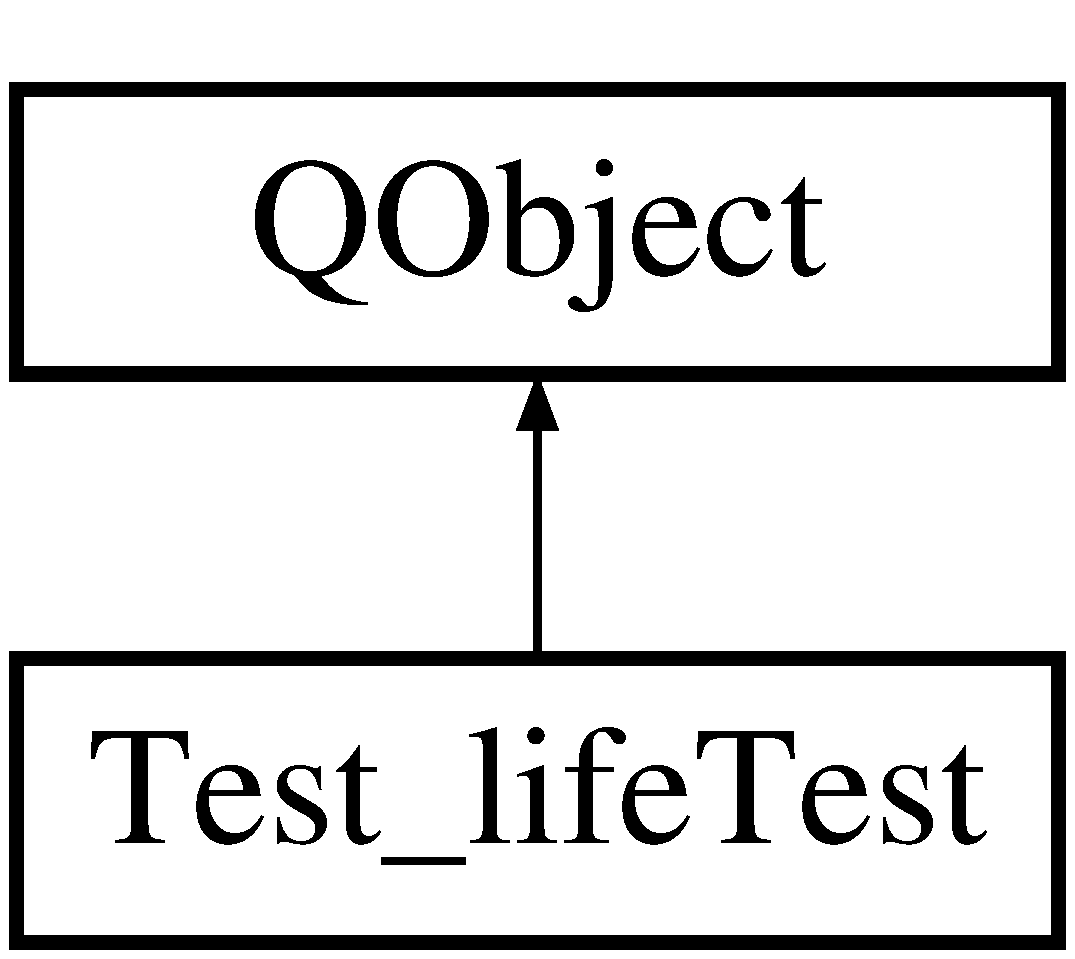
\includegraphics[height=2.000000cm]{class_test__life_test}
\end{center}
\end{figure}


The documentation for this class was generated from the following file\+:\begin{DoxyCompactItemize}
\item 
tst\+\_\+test\+\_\+lifetest.\+cpp\end{DoxyCompactItemize}

%--- End generated contents ---

% Index
\backmatter
\newpage
\phantomsection
\clearemptydoublepage
\addcontentsline{toc}{chapter}{Index}
\printindex

\end{document}
